\documentclass[a4paper]{jpconf}
\bibliographystyle{iopart-num}
\usepackage{graphicx}
\usepackage{hyperref}
\usepackage{cleveref}
\usepackage{amsmath}
\usepackage[font=small,labelfont=bf]{caption}
\begin{document}

\crefname{equation}{Equation}{Equations}
\crefname{chapter}{Chapter}{Chapters}
\crefname{section}{Section}{Sections}
\crefname{appendix}{Appendix}{Appendices}
\crefname{enumi}{Item}{Items}
\crefname{footnote}{Footnote}{Footnotes}
\crefname{figure}{Figure}{Figures}
\crefname{table}{Table}{Tables}
\crefname{theorem}{Theorem}{Theorems}
\crefname{lemma}{Lemma}{Lemmas}
\crefname{corollary}{Corollary}{Corollaries}
\crefname{proposition}{Proposition}{Propositions}
\crefname{definition}{Definition}{Definitions}
\crefname{result}{Result}{Results}
\crefname{example}{Example}{Examples}
\crefname{remark}{Remark}{Remarks}
\crefname{note}{Note}{Notes}

\title{Numerical simulation of turbulent flow in a cyclonic separator}

\author{Dmitry Bogdanov and Sergey Poniaev}

\address{Division of Plasma Physics, Atomic Physics and Astrophysics, Ioffe Physical Technical Institute, 26 Polytekhnicheskaya, St Petersburg 194021, Russian Federation}

\ead{\href{mailto:dimyriy.bogdanov@gmail.com}{dimyriy.bogdanov@gmail.com}}

\begin{abstract}
In this study a numerical simulation of turbulent flow of an air with dispersed particles is presented for cyclonic separator. Since the separator construction make it difficult to simulate the flow using the conventional turbulent models due to high streamlines curvature, the curvature correction term was included in $k-\omega-SST$ turbulence model. Experimental data for turbulent flow in U-duct has been used for model validation. The numerical simulation results demonstrate that the implemented turbulence model successfully predicts the cyclonic separator efficiency.
\end{abstract}

\section{Introduction}
Cyclonic separators are widely used for gas separation from dispersed phase. Its efficiency calculated by dividing the number of filtered particles by the total number of particles. However, numerical simulation of the turbulent flow in separator for prediction of its efficiency is a very difficult problem since conventional eddy-viscosity models can't adequately predict the flow\cite{ShurSpallart} due to high streamlines curvature and more specifically, inadequate calculation of turbulence kinetic energy production. The production can be corrected using Shur-Spalart curvature correction function for Spalart-Allmaras turbulence model reformulated\cite{Smirnov} in terms of the $k-\omega-SST$ turbulence model.

\section{Cyclonic separator model}
The typical scheme of the air flow in cyclonic separator is presented on \cref{fig:physicalModel}. The air with dispersed particles enters the cyclone through air inlet. Under the centrifugal forces the heavy particles pass near to the boundary layer on a sidewall. It that region the influence of the air flow on particles movement is relatively small in compare with influence of the gravity forces and particles falling down to the dust. Cleaner air goes out from cyclone through air outlet.
\section{SST with curvature correction model formulation}
\label{sec:model}
The correction function \eqref{eq:1} suggested in \cite{ShurSpallart} used as a multiplier of the production term in the Spalart-Allmaras eddy viscosity transport equation.

\begin{equation}
\label{eq:1}
f_{rotation} = (1+c_{r_1}) \frac{2r^*}{1+r^*} [1-c_{r_3}\tan^{-1}(c_{r_2}\tilde{r})] -c_{r_1}
\end{equation}
\begin{figure}[h]
\begin{minipage}{14pc}
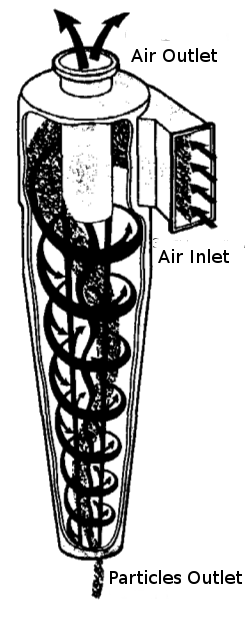
\includegraphics[width=8pc]{flowScheme1.png}\hspace{6pc}
\caption{\label{fig:physicalModel}Scheme of the air flow inside cyclonic separator.}
\end{minipage}
\begin{minipage}{20pc}
Article \cite{Smirnov} suggests to use this function as follows in respect to the SST model.

\begin{equation}
\label{eq:2}
\frac{\partial (\rho k)}{\partial t} + \frac{\partial (\rho u_j k)}{\partial x_j} = P_k f_{r_1} - \beta^* \rho k \omega + \frac{\partial}{\partial x_j} \left[ \mu_{eff}\frac{\partial k}{\partial x_j} \right]
\end{equation}

\begin{equation}
\frac{\partial (\rho \omega)}{\partial t} + \frac{\partial (\rho u_j \omega)}{\partial x_j} = \alpha \frac{\rho P_k}{\mu_t}f_{r_1}  - D_{\omega} + Cd_{\omega} + \frac{\partial}{\partial x_j} \left[ \mu_{eff}\frac{\partial \omega}{\partial x_j} \right]
\end{equation}

\begin{equation}
f_{r_1} = \max\left[ \min(f_{rotation}, 1.25), 0 \right]
\end{equation}

\begin{equation}
r^*=\frac{S}{\Omega}
\end{equation}

\end{minipage}
\end{figure}
\begin{equation}
\tilde{r} = 2\Omega_{ik}S_{jk}\left[ \frac{DS_{ij}}{Dt} + \left( \varepsilon_{imn}S_{jn} + \varepsilon_{jmn}S_{in} \right)\Omega^{rot}_m \right]\frac{1}{\Omega D^3}
\end{equation}

 \begin{equation}
 S_{ij} = \frac{1}{2}\left( \frac{\partial u_i}{\partial x_j} + \frac{\partial u_j}{\partial x_i} \right)
 \end{equation}

\begin{equation}
\Omega_{ij} = \frac{1}{2}\left( \left( \frac{\partial u_i}{\partial x_j} - \frac{\partial u_j}{\partial x_i}  \right) +2\varepsilon_{mji} \Omega^{rot}_m \right)
\end{equation}

\begin{equation}
S^2 = 2S_{ij}S_{ij}, \quad 
\Omega^2 = 2\Omega_{ij}\Omega_{ij}
\end{equation}

\begin{equation}
D^2 = \max(S^2, 0.09\omega^2)
\end{equation}

$DS_{ij}/Dt$ - components of the Lagrangian strain tensor derivative.

$$
c_{r_1} = 1.0, \quad c_{r_2} = 2.0, \quad c_{r_3} = 1.0
$$


\section{Model validation}

Turbulence model described in \cref{sec:model} has been implemented using OpenFOAM{\textregistered} mathematical library. Numerical simulation results comparison with Monson \cite{Monson} experimental data for turbulent flow in U-duct and numerical simulation in ANSYS Fluent{\textregistered} for the velocity projections $U_x$ and $U_y$ shown in \cref{fig:x0up,fig:x0down,fig:x1up,fig:x1down}. U-duct geometric and flow parameters shown in \cref{table:1}. Flow scheme presented in \cref{fig:uDuctScheme}. At the inlet section in accordance with the experiment the flow was assumed fully developed. So inlet profiles used as inlet boundary condition were obtained from preliminary computations of the turbulent flow in a plane channel.

It can be seen that the results of numerical simulation obtained using both implemented model and ANSYS Fluent{\textregistered} solver are in good agreement with the Monson experimental data. SST model with curvature correction shows significant improvement of simulated velocity profile compared to the non-modified SST model.
\begin{figure}[h]
\begin{minipage}{15pc}
\begin{center}
\captionof{table}{\label{table:1} Geometric and flow parameters for air flow in U-duct.}
\begin{tabular}{{r}{l}}
\br
Channel height, $H$ & $3.81cm$\cr
Channel length, $L$ & $10H$\cr
Inner radius, $R_i$ & $1.91cm$\cr
Outer radius, $R_o$ & $5.72cm$\cr
Average velocity at inlet $U_{in}$ & $30.1m/s$\cr
Average temperature at inlet, $T_{in}$ & $264K$\cr
Pressure at outlet, $p_{out}$ & $1.15atm$\cr
Reynolds number, Re & $~10^5$\cr
\end{tabular}
\end{center}
\end{minipage}\hspace{3pc}
\begin{minipage}{20pc}
\begin{center}
\includegraphics[width=20pc]{UDuct.eps}
\captionof{figure}{\label{fig:uDuctScheme} Scheme of air flow in U-duct}
\end{center}
\end{minipage}
\end{figure}
\begin{figure}[ht]
	\begin{minipage}{0.45\linewidth}
		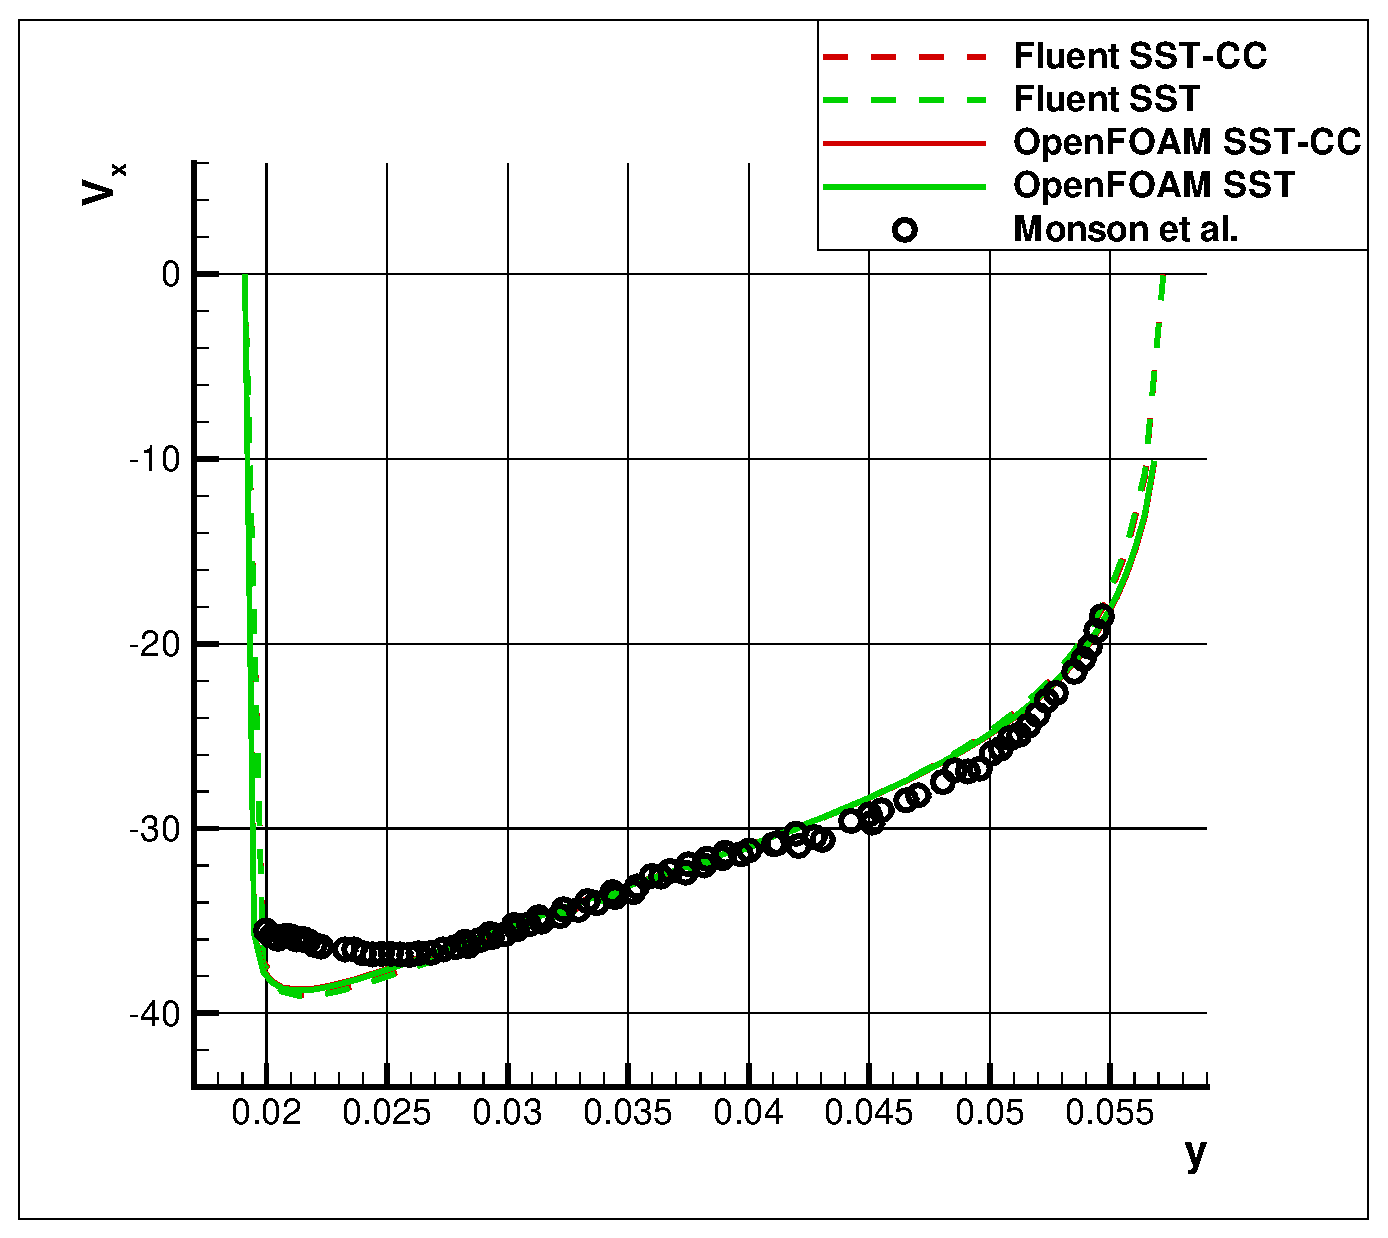
\includegraphics[scale=0.33]{xh0up}
		\caption{$U_x$, $x/H=0$ (lower channel)}
		\label{fig:x0up}
	\end{minipage}
	\hspace{0.5em}
	\begin{minipage}{0.45\linewidth}
		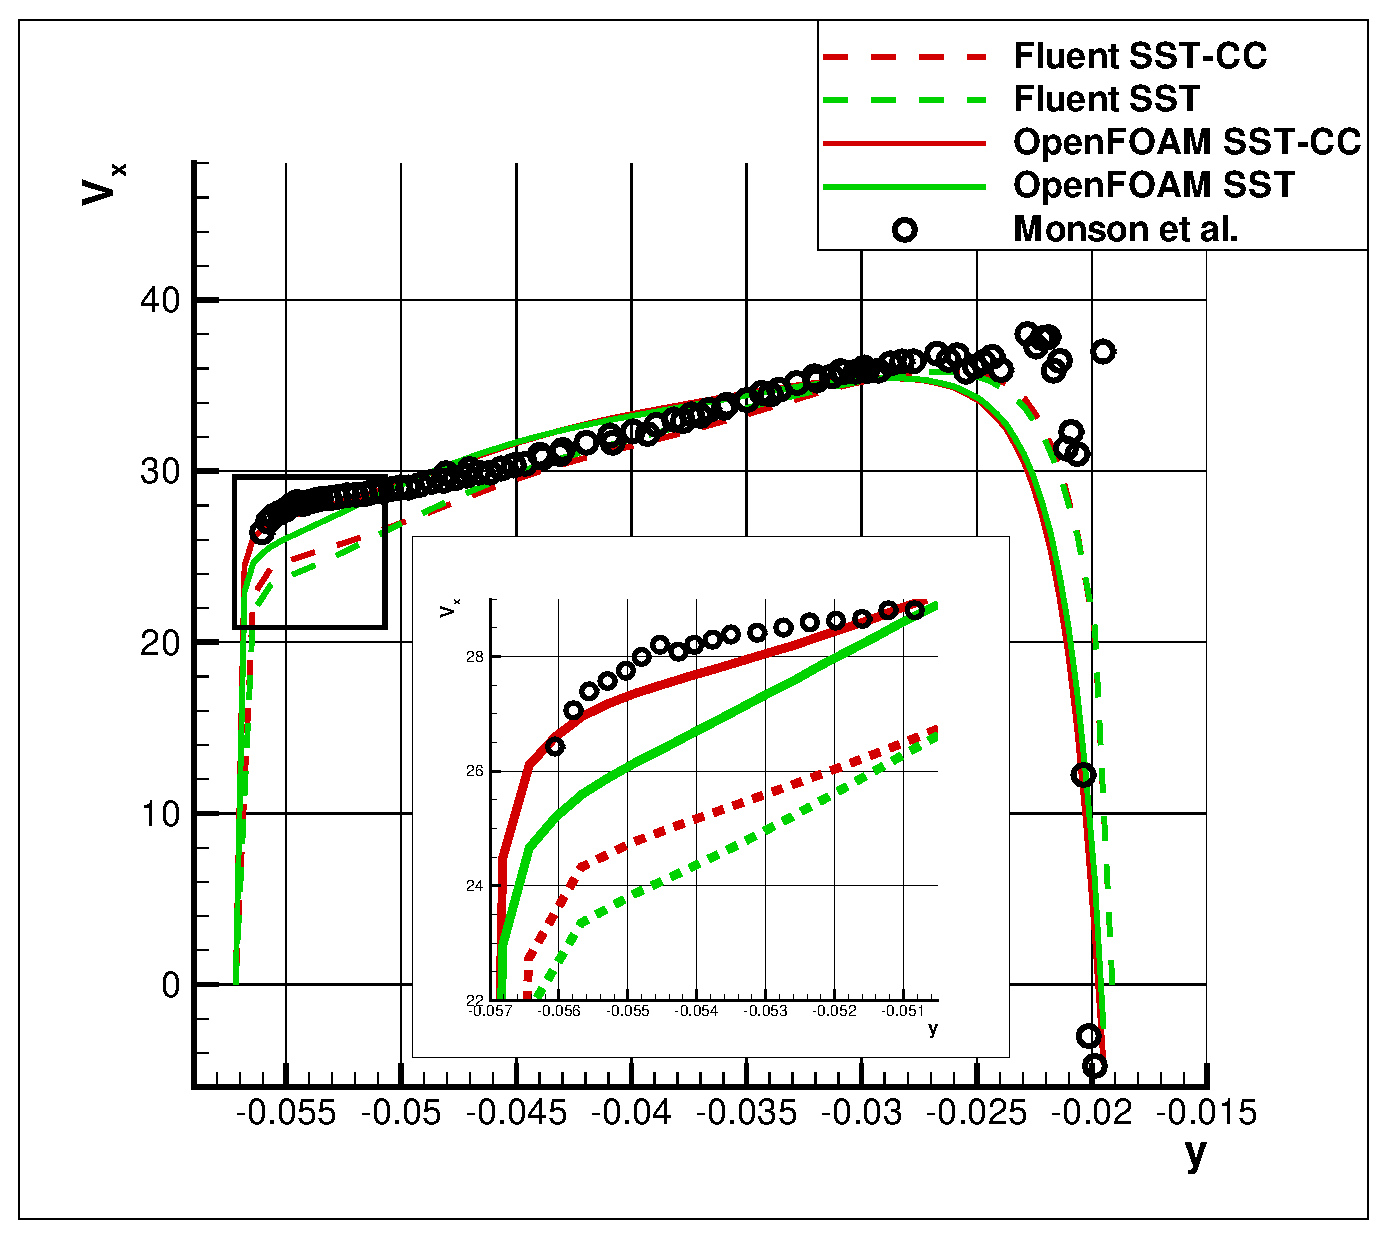
\includegraphics[scale=0.33]{xh0down}
		\caption{$U_y$, $x/H=0$ (top channel)}
		\label{fig:x0down}
	\end{minipage}
\end{figure}
\begin{figure}[ht]
	\vspace{-1em}
	\begin{minipage}{0.45\linewidth}
		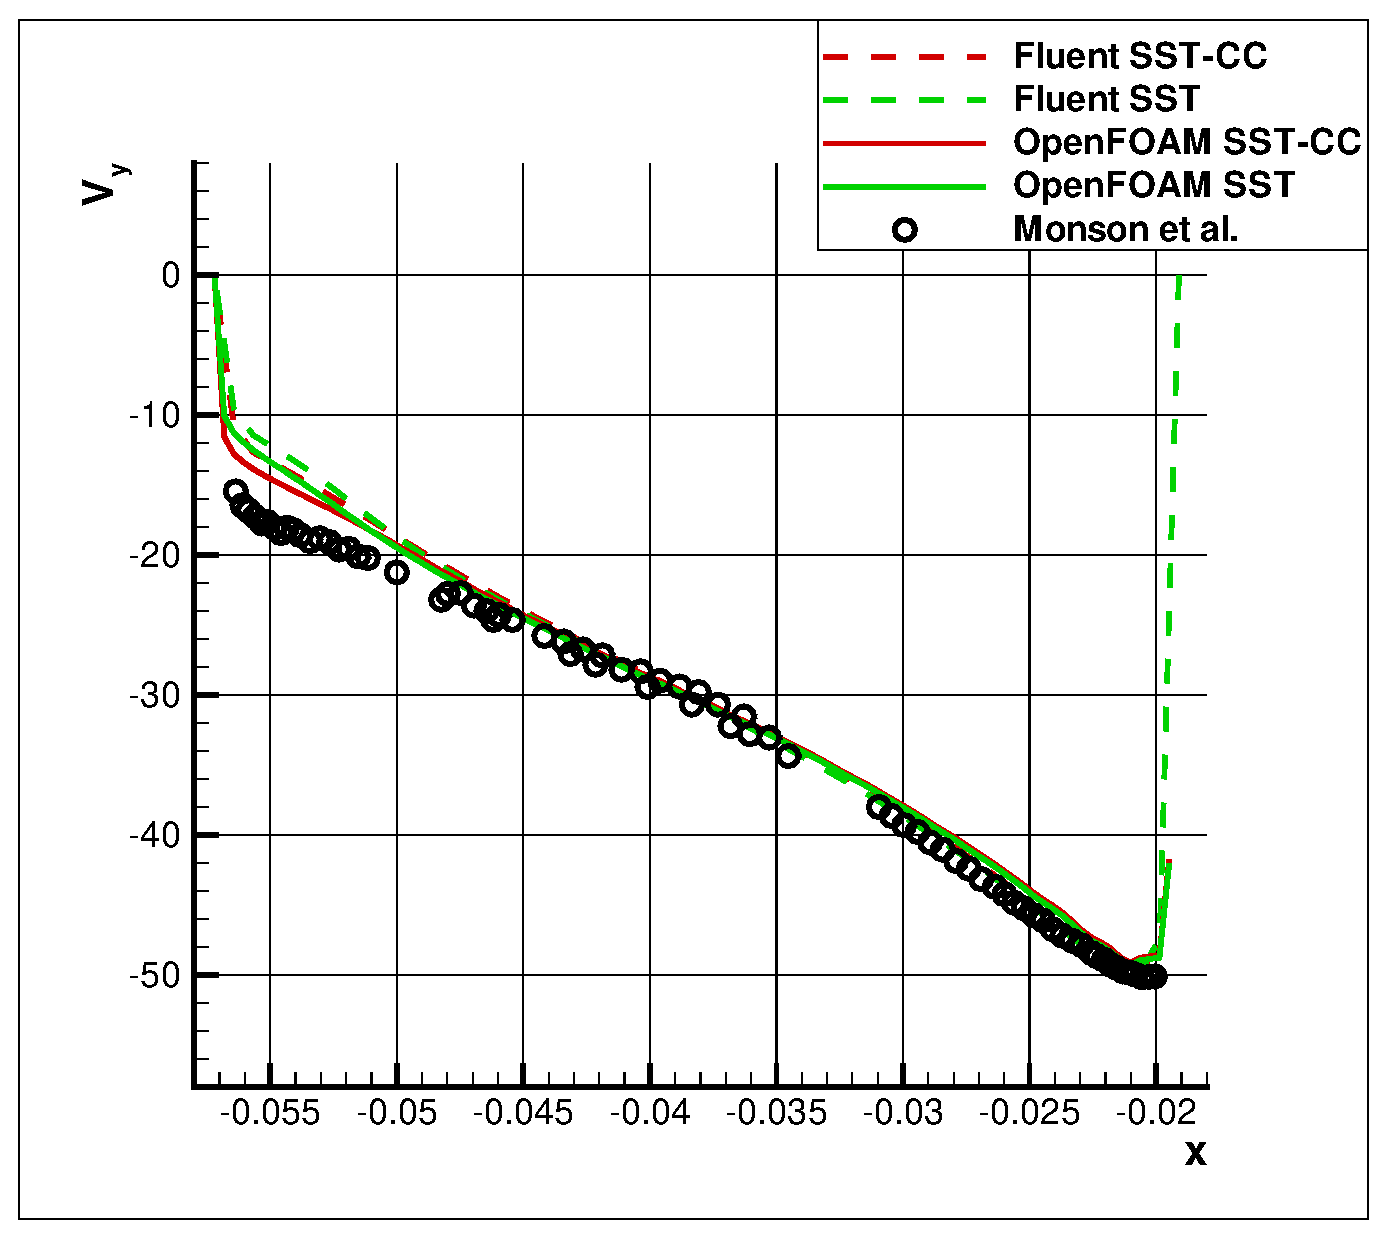
\includegraphics[scale=0.33]{yh0}
		\caption{$U_y$, $y/H=0$}
		\label{fig:x1up}
	\end{minipage}
	\hspace{0.5em}
	\begin{minipage}{0.45\linewidth}
		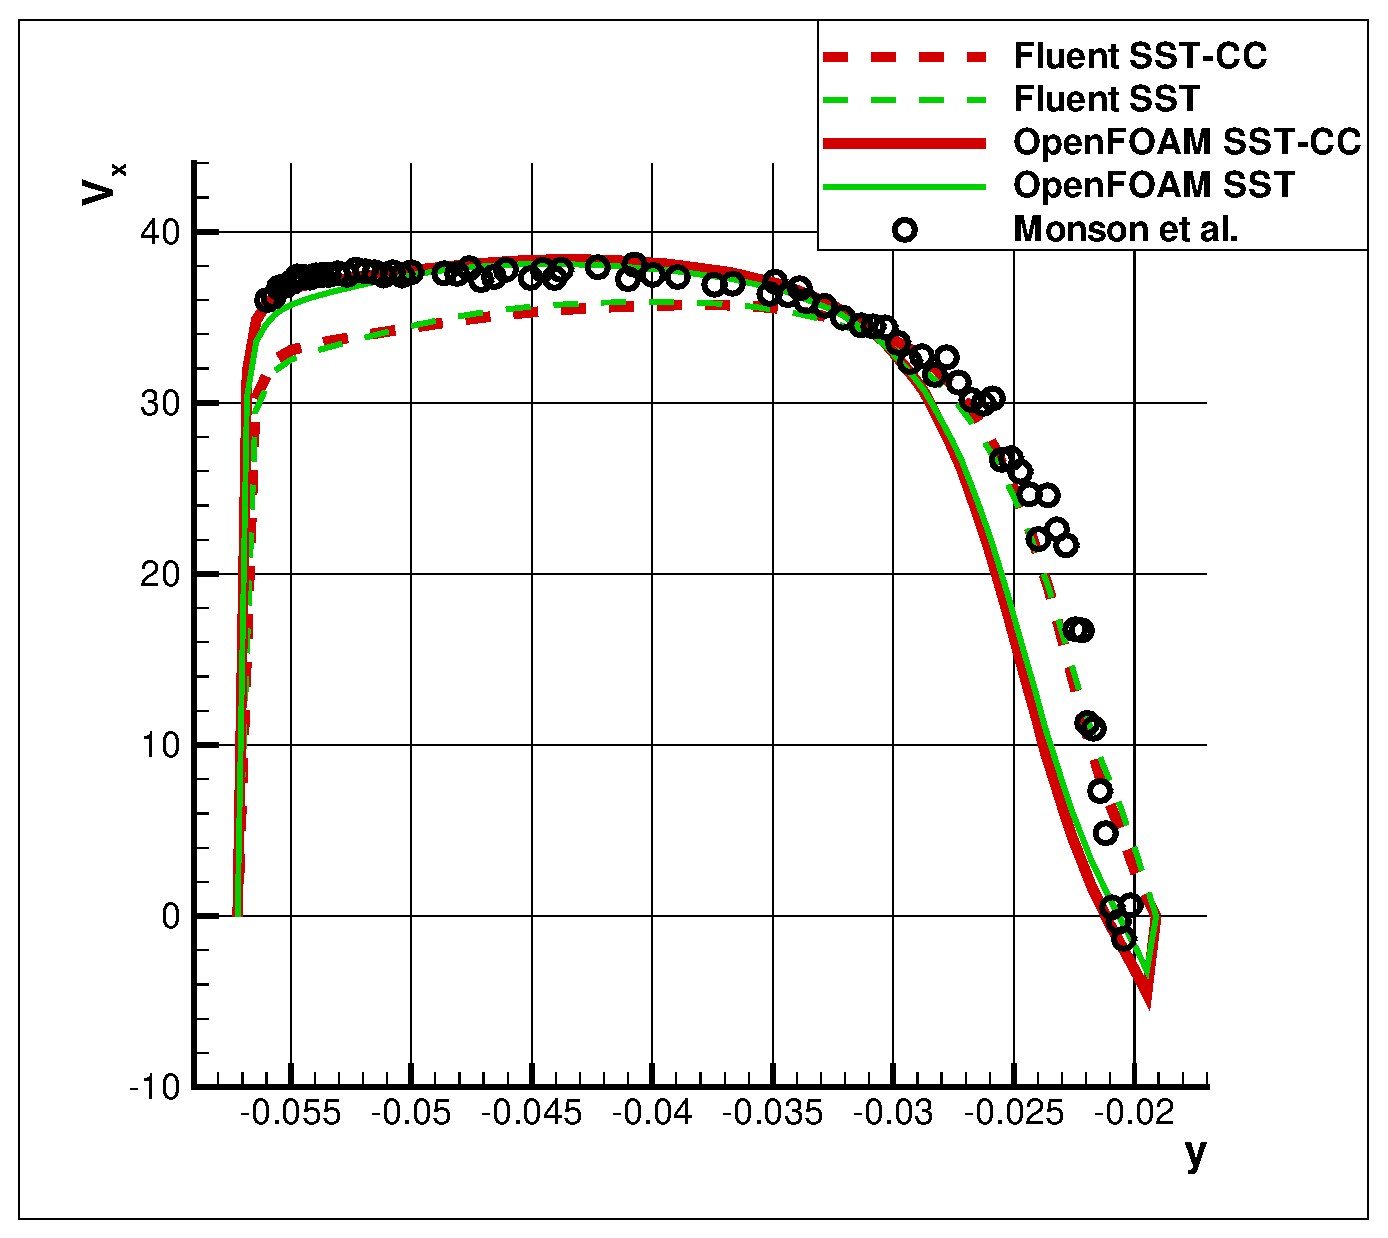
\includegraphics[scale=0.33]{xh1down}
		\caption{$U_x$, $x/H=1$}
		\label{fig:x1down}
	\end{minipage}
\end{figure}
\section{Results}

In this section we consider the flow in cyclonic separator shown in \cref{fig:cycloneGeometryScheme}. Geometric parameters and boundary conditions presented in \cref{cycloneGeomPar} and \cref{geometrytable} respectively. Inlet velocity profile obtained from computation of fully developed turbulent flow in square-section channel.

Solution has been obtained for three different velocities and three different particle diameters. Results of the numerical simulation, compared with the Dirgo and Leith\cite{DirgoLeith} experimental data presented in \cref{tableSolution}. As can be seen from the table, results of the numerical simulation are in good agreement with the experimental data. As might be expected, cyclone efficiency degrades in direct ratio with particles diameter. For diameter $\le 10^{-7}m$ cyclone is not applicable at all, but for diameter $\ge 10^{-5}m$ it shows almost $100\%$ efficiency. With the decrease of the inlet velocity, cyclone efficiency also degrades due to decreasing influence of a centrifugal force.

Results of particle distribution presented in \cref{fig:parcelsCyclone1,fig:parcelsCyclone3}. Particles with diameter $\le 10^{-7}$ almost uniformly distributed inside filter which apparently means that influence of centrifugal forces is not large enough to filter out significant part of particles. In opposite, particles with diameters $\ge 10^{-5}$ distributed mostly inside boundary layer on filter sidewall and can be filtered out.

According to the calculation results we can make a conclusion that curvature correction function, suggested in \cite{ShurSpallart}, reformulated in \cite{Smirnov} and implemented using OpenFOAM in current paper, can be successfully used for simulation of turbulent flows with high streamlines curvature.

\begin{minipage}{0.6\textwidth}
    \captionof{table}{Cyclone geometric parameters}
    \label{cycloneGeomPar}
			\begin{tabular}{r l}
				\hline
				\label{geometrytable}
				Cylinder diameter,& $D=0.205m$ \\
				Outlet diameter,& $D_e=0.5D$ \\
				Inlet channel height,& $a=0.5D$ \\
				Inlet channel width,& $b=0.2D$ \\
				Inlet channel length,& $h_e=0.75D$ \\
				Total filter height,& $H=4.0D$ \\
				Cylinder height,& $h=1.5D$ \\
				Lower section diameter,& $B=0.36D$ \\
				Dust height,& $h_d=0.25D$ \\
				Dust diameter,& $D_d=0.75D$ \\
			\end{tabular}
			\vspace{1pc}
			\captionof{table}{Cyclone Flow parameters}
    \label{cycloneBC}
	\begin{tabular}{r l}
		\hline
		\label{geometrytable}
		Inlet velocity, &$U_{in}=$  $5, 10, 15, 20 m/s$ \\
		Inlet temperature,& $T_{in}=$  $300 K$ \\
		Particles temperature,& ${T_p}_{in}=$  $T_{in}$ \\
		Particles inlet velocity,& ${U_p}_{in} = U_{in}$ \\
		Outlet pressure,& $P_{out}=$  $1atm$ \\
		Wall heat transfer,& $q_w=$  $0$ \\
		Particles diameters,& $d_p \sim $ $10^{-5}m, 10^{-6}m, 10^{-7}	m$\\
	\end{tabular}
    \end{minipage}
    \hspace{1em}
  \begin{minipage}{0.35\textwidth}
    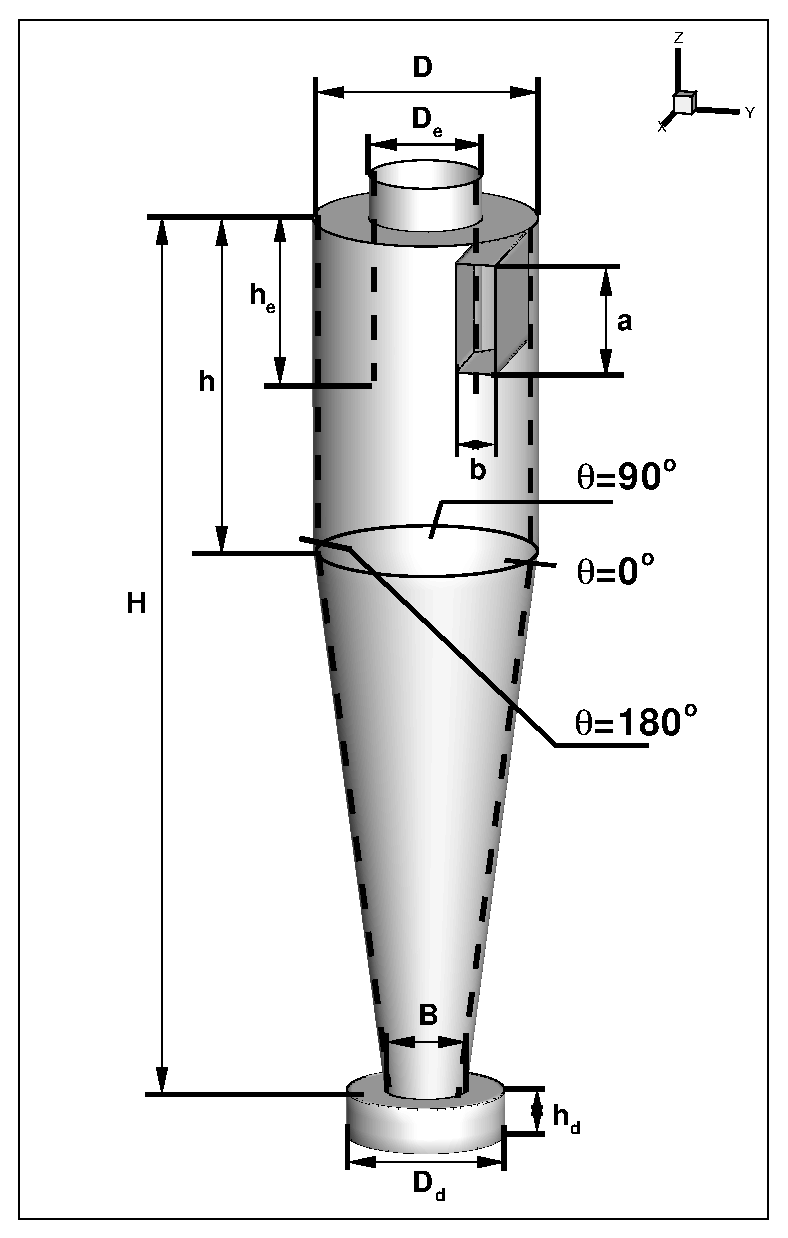
\includegraphics[scale=0.45]{cycloneGeometryTeta}
	\captionof{figure}{Cyclone scheme}
	\label{fig:cycloneGeometryScheme}
  \end{minipage}
\begin{table}[h]
\begin{center}
		\caption{Cyclonic separator efficiency $\eta$ comparison}
		\label{tableSolution}
		\begin{tabular}{|c|c|c|}
			\hline
			Flow parameters & $\eta$, Numerical simulation & $\eta$, Experiment\\
			\hline
			$U_{in}=20m/s, d=5 \cdot 10^{-5}m$ & 100\% & 100\% \\
			\hline
			$U_{in}=20m/s, d=5 \cdot 10^{-6}m$ & 93\% & 90\%\\
			\hline
			$U_{in}=20m/s, d=5 \cdot 10^{-7}m$ & 27\% & 10\%\\
			\hline
			$U_{in}=15m/s, d=10^{-5}m$ & 80\% & 90\% \\
			\hline
			$U_{in}=10m/s, d=10^{-5}m$ & 72\% & 85\% \\
			\hline
			$U_{in}=5m/s, d=10^{-5}m$ & 75\% & 80\% \\
			\hline
		\end{tabular}
\end{center}
	\end{table}
	\newpage
\begin{figure}[h]
	\begin{minipage}{0.475\linewidth}
		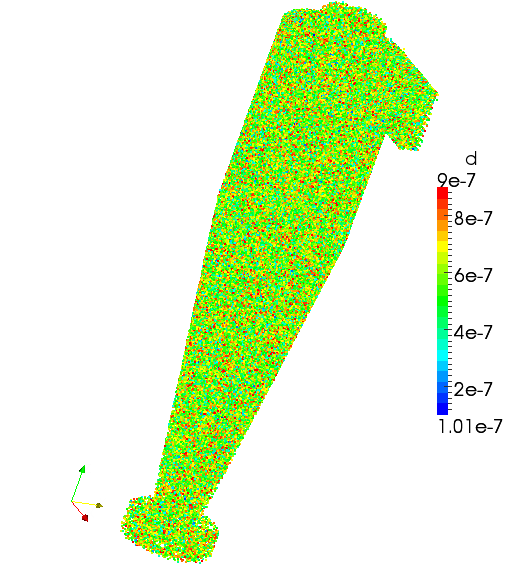
\includegraphics[scale=0.4]{parcelsCyclone1}
		\caption{Particles distribution for $d \sim 10^{-7}$ и $U_{in} = 20m/s$}
		\label{fig:parcelsCyclone1}
	\end{minipage}
	\hspace{0.5em}
	\begin{minipage}{0.475\linewidth}
		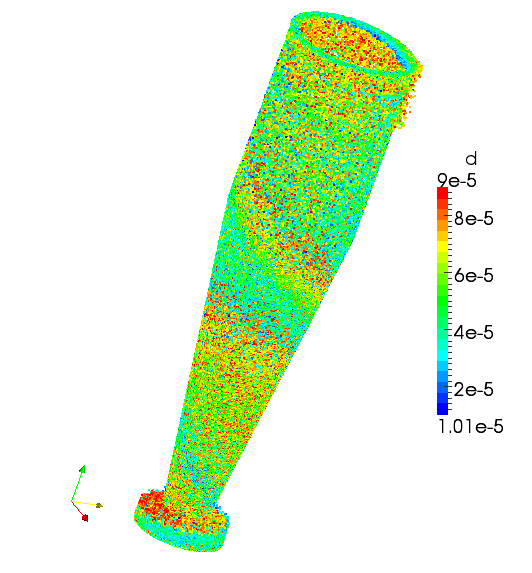
\includegraphics[scale=0.4]{parcelsCyclone3}
		\caption{Particles distribution for $d \sim 10^{-5}$ и $U_{in} = 20m/s$}
		\label{fig:parcelsCyclone3}
	\end{minipage}
\end{figure}	
\section*{References}
\bibliography{iopart-num}
\end{document}


